\section{Istruzioni d'uso}

Si consiglia di leggere prima le istruzioni per gli utenti non autenticati e successivamente quelle per gli utenti autenticati, in quanto l'accesso è simile per clienti e ristoratori, mentre alcune funzionalità come l'esplorazione sono disponibili solo per i clienti autenticati.

\subsection{Utente non autenticato} % --------------------- SECTION DEL UTENTE NON AUTENTICATO ---------------------%
Come utente non autenticato, hai accesso a una serie di funzionalità di base che ti permettono 
di esplorare EasyMeal e di accedere o registrarti.

\subsubsection{Navigazione}
La barra di navigazione in alto ti permette di accedere facilmente alle varie sezioni della piattaforma. 
Puoi tornare alla schermata principale cliccando sul logo EasyMeal o sul nome EasyMeal entrambi posti in alto a sinistra.


\begin{figure}[htbp]
    \centering
    \adjustbox{width=0.375\textwidth, frame, center}{
\includegraphics{./img/BarraNavigazioneClienteNonAutenticato.jpg}}
    \caption{Barra di Navigazione per l'utente non autenticato}
    %  \label{fig:esempio1}
\end{figure}


\subsubsection{Home Page}
La Home Page è il punto di ingresso principale per gli utenti non autenticati. 
Qui troverai informazioni su EasyMeal, inclusi dettagli su cosa offre la piattaforma, 
quali problemi risolve e come funziona. 
La Home Page presenta anche una barra di navigazione che ti permette di accedere alle sezioni di login, registrazione ed esplorazione.

\subsubsection{Login}
Per accedere come utente autenticato, utilizza il form di accesso presente nella HomePage oppure nella barra di navigazione. 
Inserisci la tua email e la password corrispondente.

Se l'autenticazione avviene con successo, riceverai una notifica in basso a destra indicante ``Utente autenticato''.

Se ci sono errori durante l'autenticazione, come credenziali errate o account non esistente, verranno visualizzati messaggi di errore appropriati.

Se non hai ancora un account, puoi registrarti cliccando sul link ``Registrati subito''  sotto il form di accesso.

\begin{figure}[htbp]
    \centering
    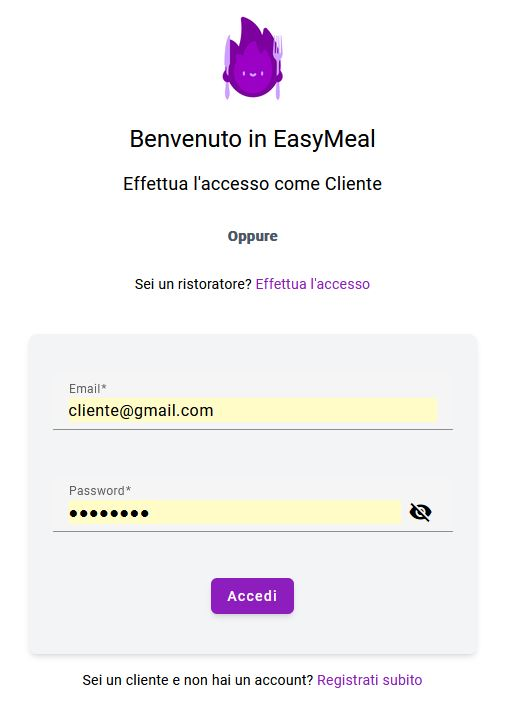
\includegraphics[width=0.375\textwidth]{./img/Login.jpg}
    \caption{Form di login}
    % \label{fig:esempio2} 
\end{figure}

Si noti che i vari campi del form danno anche un feedforward in base alla correttezza dei dati inseriti. 
Una volta che l'utente inserisce i campi obbligatori segnalati con un asterisco è possibile cliccare sul pulsante ``Accedi'' per procedere con l'autenticazione.

\subsubsection{Registrazione cliente}
Per registrarti come nuovo cliente, compila il form di registrazione con il tuo nome, cognome, email e password desiderati. 
Una volta completato il form e inviata la richiesta di registrazione, riceverai una notifica in basso a destra indicante 
``Utente creato con successo'' se la registrazione è avvenuta con successo.

Altrimenti, verranno visualizzati messaggi di errore se ci sono problemi durante il processo di registrazione, come ``Utente già esistente'' o ``Richiesta fallita''.

\begin{figure}[H]
    \centering
    \includegraphics[width=0.375\textwidth]{./img/RegistrazioneCliente.jpg}
    \caption{Form di registrazione come cliente}
    % \label{fig:esempio3}
\end{figure}

\subsubsection{Registrazione ristoratore}
Per registrarti come nuovo ristoratore, compila il form di registrazione con il tuo nome e cognome del proprietario, nome del ristorante,
email e password desiderati, numero di telefono e indirizzo fisico del ristorante, posti a sedere e costo, indirizzo del sito web relativo al 
ristorante se lo si ha, e anche una breve descrizione se si desidera. 
Si noti che per il numero di telefono bisogna inserire tutto attaccato il prefisso e poi il numero, ad esempio (+313319999999).
Mentre per il costo bisogna indicarlo con un valore compreso tra 0 e 3, dove 3 indica un costo elevato e 0 un costo basso.
Una volta completato il form e inviata la richiesta di registrazione, riceverai una notifica in basso a destra indicante 
``Utente creato con successo'' se la registrazione è avvenuta con successo.

Altrimenti, verranno visualizzati messaggi di errore se ci sono problemi durante il processo di registrazione, come ``Utente già esistente'' o ``Richiesta fallita''.

\begin{figure}[htbp]
    \centering
    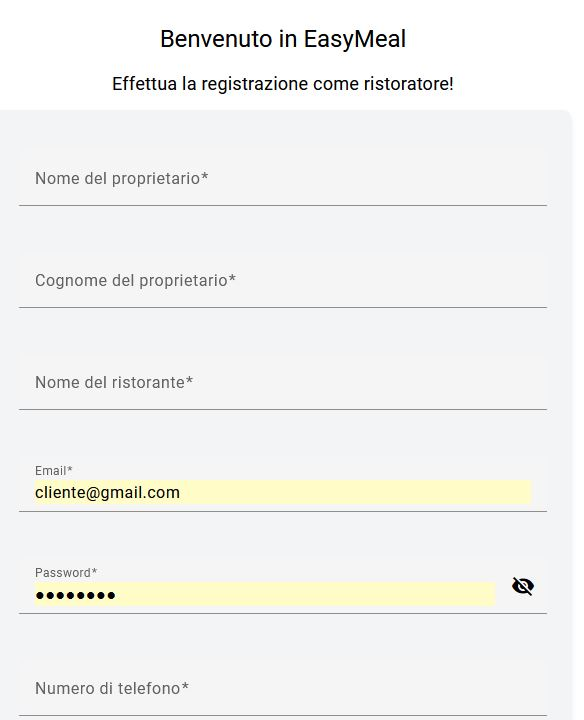
\includegraphics[width=0.375\textwidth]{./img/RegistrazioneRistoratore1.jpg}
    \hfill
    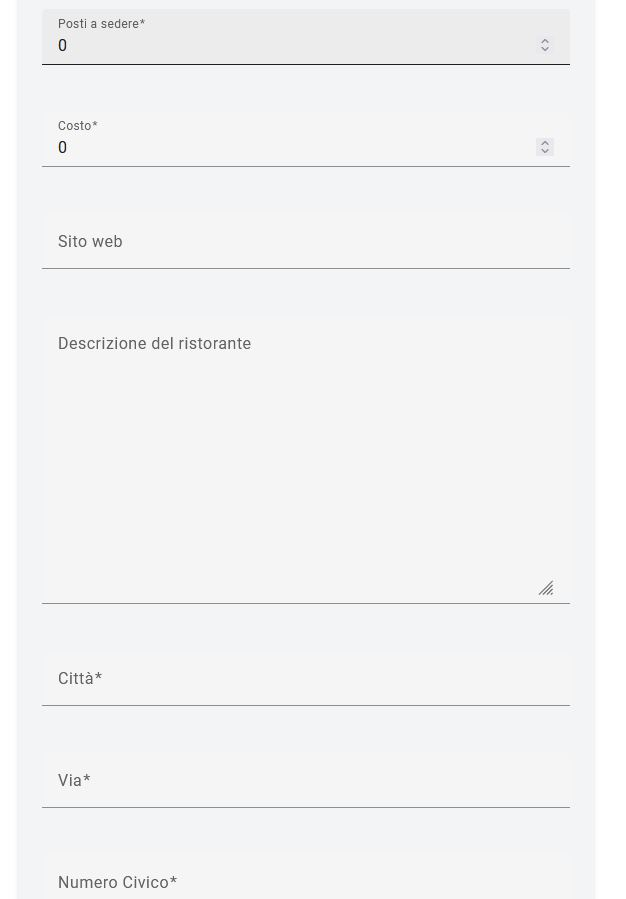
\includegraphics[width=0.375\textwidth]{./img/RegistrazioneRistoratore2.jpg}
    \hfill
    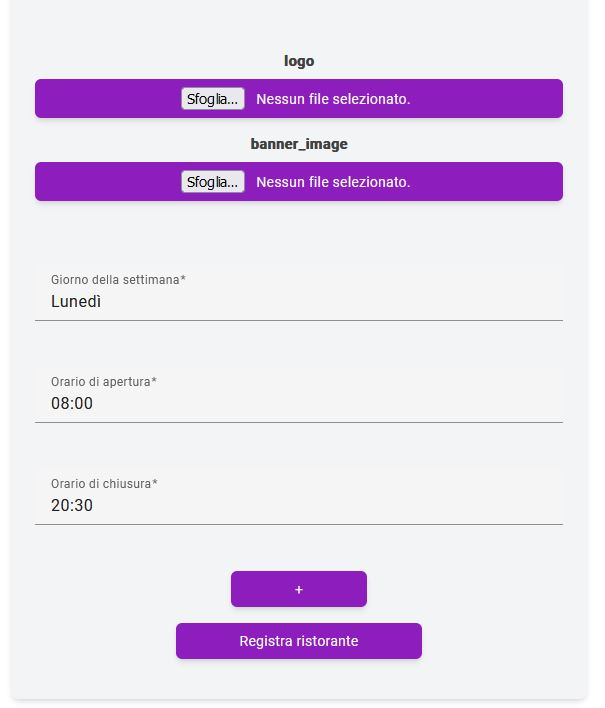
\includegraphics[width=0.375\textwidth]{./img/RegistrazioneRistoratore3.jpg}
    \caption{Form di registrazione come ristoratore}
    % \label{fig:esempio4}
\end{figure}

Inoltre è possibile inserire immagini per caricare il logo visualizzabile del ristorante e il relativo banner.
Inoltre è possibile inserire per ciascun giorno della settimana l'orario di apertura e chiusura del ristorante.
Una volta inserito per un giorno l'orario di apertura e chiusura, è possibile cliccare sul pulsante ``+'' per aggiungere un altro giorno.
Una volta cliccato sul pulsante ``+'' sarà visualizzabile sopra lo stesso pulsante tutti gli orari inseriti fino ad ora e voledno è possibile 
rimuoverli cliccando sul pulsante ``X'' che compare non appena si avrà inserito almeno un giorno con relativo orario.
Per tutto ciò consultare la immagine del form di registrazione come ristoratore parte3.



\subsubsection{Esplora}
La sezione ``Esplora'' ti permette di cercare, filtrare e visualizzare tutti i ristoranti registrati su EasyMeal. 
Utilizza la barra di ricerca per inserire il nome del ristorante e usare il pulsante ``Cerca'' per avviare la ricerca.

\begin{figure}[htbp]
    \centering
    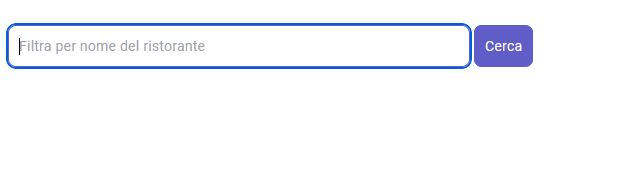
\includegraphics[width=0.375\textwidth]{./img/EsploraClienteNonAutenticato.jpg}
    \caption{Pagina di esplorazione dei ristoranti per l'utente non autenticato}
    % \label{fig:esempio5}
\end{figure}

Se non si applica un filtro attraverso la barra di ricerca, verranno visualizzati tutti i ristoranti registrati su EasyMeal.

\subsubsection{Visualizza in dettaglio un ristorante}
Inoltre è possibile per ciascun ristorante cliccare sul link ``Dettaglio'' per visualizzare in dettaglio tutte le informazioni relative al ristorante.

\begin{figure}[htbp]
    \centering
    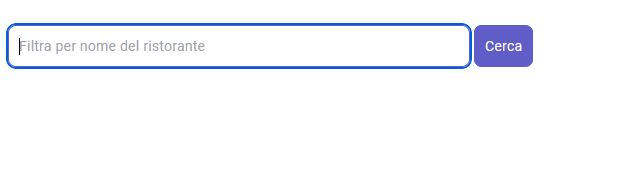
\includegraphics[width=0.375\textwidth]{./img/Dettaglio.jpg}
    \caption{Bottone di visualizzazione in dettaglio di un ristorante}
    % \label{fig:esempio6}
\end{figure}

Nella seguente pagina sarà possibile visualizzare tutte le informazioni relative al ristorante (le stesse presenti nel form di registrazione come ristoratore) 
e inoltre sarà possibile visualizzare il menu del ristorante, con i relativi piatti e prezzi e inoltre visualizzare le recensioni del ristorante.

\begin{figure}[htbp]
    \centering
    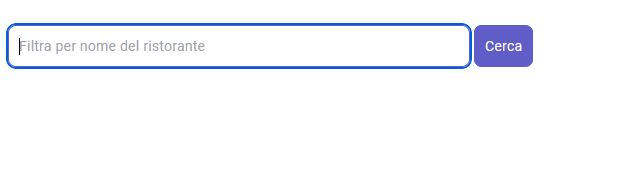
\includegraphics[width=0.375\textwidth]{./img/VisualizzaDettagliRistorante.jpg}
    \caption{Pagina di visualizzazione in dettaglio relative ad un ristorante}
    % \label{fig:esempio7}
\end{figure}























\subsection{Cliente} % --------------------- SECTION DEL CLIENTE ---------------------%

 
\subsubsection{Home Page}
Una volta effettuato l'accesso come cliente, verrai reindirizzato alla tua Home Page personale.
Questa Home Page è praticamente identica a quella degli utenti non autenticati, ma con modifiche 
relative alla barra di navigazione in alto. 


\subsection{Barra di navigazione}
La barra di navigazione in alto ti permette di accedere alle sezioni di esplorazione dei ristoranti, 
visualizzare e gestire le proprie prenotazioni, controllare e leggere le notifiche ricevute ed effettuare il ``logout''.

\subsubsection{Esplora}
La sezione ``Esplora'' ti permette di cercare, filtrare e visualizzare tutti i ristoranti registrati su EasyMeal, 
e andare in dettaglio per visualizzare tutte le informazioni relative ad un ristorante. Esattamente come un utente non autenticato.

Una volta entrati nel dettaglio di un ristorante, c'è un'aggiunta speciale: il bottone ``Prenota'' che ti permette di prenotare un tavolo di un ristorante, 
se c'è ancora disponibilità di posti a sedere.

\begin{figure}[htbp]
    \centering
    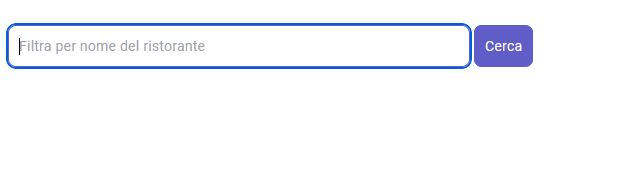
\includegraphics[width=0.5625\textwidth]{./img/Dettaglio.jpg}
    \caption{Bottone di prenotazione di un tavolo di un ristorante}
    % \label{fig:esempio8}
\end{figure}

\subsubsection{Prenotazione di un tavolo}
Una volta cliccato sul tasto prenotazione di un tavolo comparirà un form per inviare la richiesta di prenotazione che sarà accettata o rifiutata dal ristoratore.
Sarà richiesto di inserire il giorno desiderato e un orario compreso tra l'orario di apertura e chiusura del ristorante di quel relativo giorno, inoltre il numero 
di persone che saranno presenti al tavolo.

\begin{figure}[htbp]
    \centering
    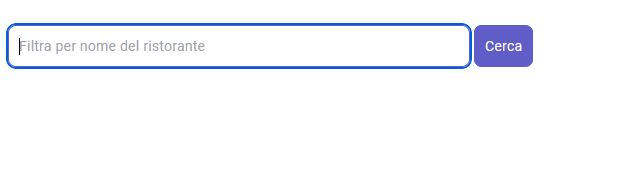
\includegraphics[width=0.5625\textwidth]{./img/Dettaglio.jpg}
    \caption{Form di richiesta di prenotazione di un tavolo di un ristorante}
   %  \label{fig:esempio9}
\end{figure}

\subsubsection{Gestione prenotazioni}
Tornando alla barra di navigazione, cliccando su ``Prenotazioni'' si accede alla pagina di gestione delle prenotazioni.
In cui si ha un elenco di tutte le prenotazioni effettuate, con la possibilità di visualizzare in dettaglio una prenotazione, semplicemente cliccando su di essa.
In questa lista si possono visualizzare le prenotazioni in attesa di conferma, quelle confermate e quelle rifiutate, quindi si possono visualizzare il nome della 
prenotazione, l'orario in cui è stata effettuata, lo stato della prenotazione e il ristorante a cui si riferisce, e lo stato della prenotazione.

\begin{figure}[htbp]
    \centering
    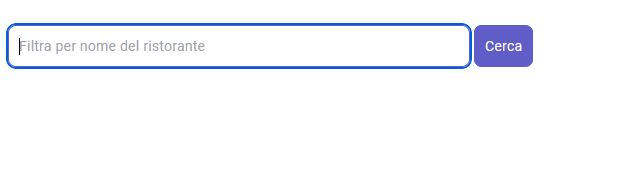
\includegraphics[width=0.5625\textwidth]{./img/Dettaglio.jpg}
    \caption{Visualizzazione delle prenotazioni effettuate}
    % \label{fig:esempio10}
\end{figure}

\subsubsection{Eliminazione prenotazione}
Nel caso in cui si è stati aggiunti ad un prenotazione e non si vuole partecipare o la si vuole cancellare bisognerà semplicemente cliccare sul pulsante ``X'' 
che compare a destra di ciascuna prenotazione nella lista.

\begin{figure}[htbp]
    \centering
    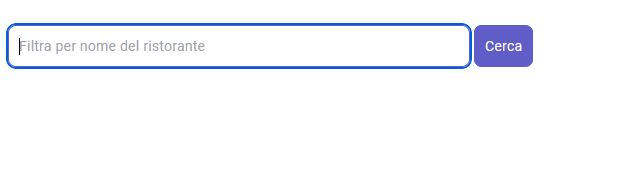
\includegraphics[width=0.5625\textwidth]{./img/Dettaglio.jpg}
    \caption{Pulsante di eliminazione di una prenotazione}
    % \label{fig:esempio11}
\end{figure}

\subsubsection{Accettazione prenotazione}
Nel caso contrario, ovvero nel caso in cui si è stati aggiunti ad una prenotazione e si desidera confermare la presenza bisognerà semplicemente cliccare sul pulsante ``V'', 
che compare a destra di ciascuna prenotazione nella lista.

\begin{figure}[htbp]
    \centering
    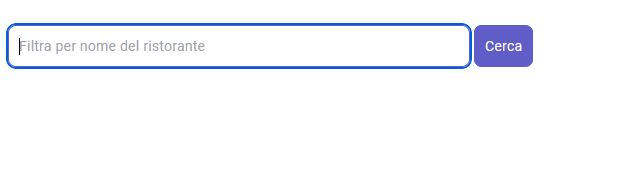
\includegraphics[width=0.5625\textwidth]{./img/Dettaglio.jpg}
    \caption{Pulsante di accettazione di una prenotazione}
    % \label{fig:esempio12}
\end{figure}

\subsubsection{Notifiche}
Tornando alla barra di navigazione, cliccando su ``Notifiche'' si accede alla pagina di visualizzazione delle notifiche.
In cui si ha la possibilità di filtrare le notifiche in base a Nuove o Lette, semplicemente cliccando sopra nuove o lette. Per default 
saranno visualizzate quelle nuove in base all'ordine di ricezione. 
Per eliminare la spunta di novità su una notifica basterà cliccare su di essa.

\begin{figure}[htbp]
    \centering
    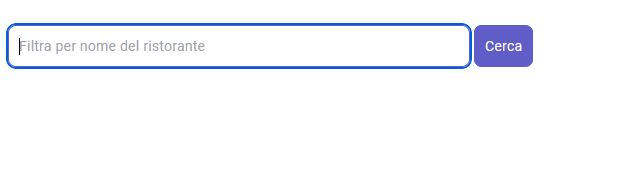
\includegraphics[width=0.5625\textwidth]{./img/Dettaglio.jpg}
    \caption{Visualizzazione delle notifiche ricevute}
    % \label{fig:esempio13}
\end{figure}

\subsubsection{Logout}
L'ultima funzionalità presente nella barra di navigazione di un cliente è la possibilità di effettuare il ``logout'' cliccando sul pulsante ``Logout''.
Una volta effettuato con successo si sarà reindirizzati nella Home Page di un classico utente non autenticato con le relative funzionalità.























\subsection{Ristoratore} % --------------------- SECTION DEL RISTORATORE ---------------------%

    \subsubsection{Home Page}
    Una volta effettuato l'accesso come ristoratore, verrai reindirizzato alla tua Home Page personale. Composta da un calendario in cui è possibile selezionare il giorno desiderato per visualizzare le prenotazioni effettuate per quel giorno. Inoltre il calendario presenta per ciascun giorno delle possibili colorazioni diverse:
        \begin{itemize}
            \item Nessun colore: indica che non ci sono prenotazioni per quel giorno.
            \item Rosso: indica che ci sono prenotazioni in attesa di conferma per quel giorno.
            \item Verde: indica che ci sono prenotazioni confermate per quel giorno.
        \end{itemize}
        
        \begin{figure}[htbp]
            \centering
            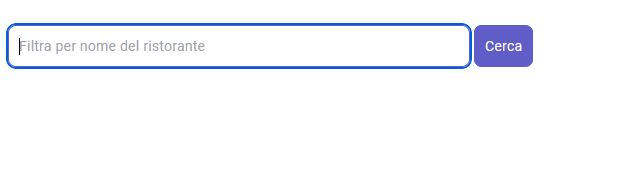
\includegraphics[width=0.5625\textwidth]{./img/Dettaglio.jpg}
            \caption{Calendario delle prenotazioni}
        \end{figure}
        
        A destra del calendario vengono visualizzate le prenotazioni effettuate del giorno selezionato, con la possibilità di visualizzare in dettaglio una prenotazione, semplicemente cliccando su di essa. Inoltre è possibile filtrarle per stato della prenotazione, orario o numero. Nella parte più a destra si hanno la lista di tutti gli ingredienti necessari a soddisfare la lista di prenotazioni visualizzata.
        
        \begin{figure}[htbp]
            \centering
            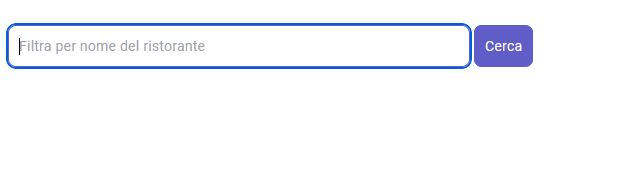
\includegraphics[width=0.5625\textwidth]{./img/Dettaglio.jpg}
            \caption{Barra di filtraggio delle prenotazioni}
        \end{figure}
        
        \begin{figure}[htbp]
            \centering
            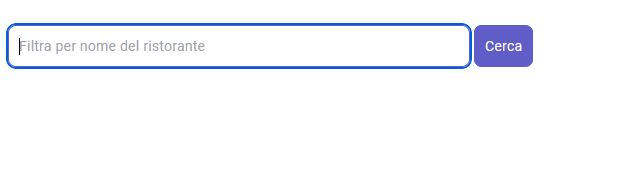
\includegraphics[width=0.5625\textwidth]{./img/Dettaglio.jpg}
            \caption{Lista degli ingredienti necessari per la giornata selezionata}
        \end{figure}

    \subsubsection{Barra di navigazione}
    La barra di navigazione in alto ti permette di accedere alle sezioni di esplorazione dei ristoranti, alla gestione delle prenotazioni, alla visualizzazione delle notifiche e al logout. Le funzionalità della barra di navigazione del ristoratore sono state precedentemente discusse nella sezione del cliente e quindi non verranno ripetute. Inoltre, la barra di navigazione del ristoratore include due funzionalità aggiuntive: "Piatti" e "Ingredienti".
        
        \begin{figure}[htbp]
            \centering
            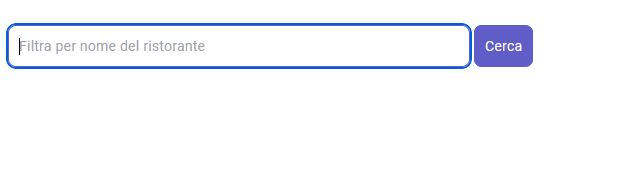
\includegraphics[width=0.5625\textwidth]{./img/Dettaglio.jpg}
            \caption{Barra di navigazione per il ristoratore}
        \end{figure}

    \subsubsection{Ingredienti}
    Questa sezione offre un'interfaccia intuitiva per la gestione degli ingredienti. Puoi inserire il nome del piatto e scegliere l'unità di misura tra le opzioni disponibili: g, ml, p, q.b. (grammi, millilitri, pezzi, quanto basta). Dopo aver inserito il nome e l'unità di misura, puoi salvare l'ingrediente al piatto. Sotto il modulo di inserimento, sono elencati tutti gli ingredienti presenti nel menu del ristorante. Puoi modificarli selezionando l'ingrediente (riconoscibile per lo sfondo celeste) e modificando i valori nel modulo, o eliminarli facendo clic sul pulsante "Elimina" a destra.
    
        \begin{figure}[htbp]
            \centering
            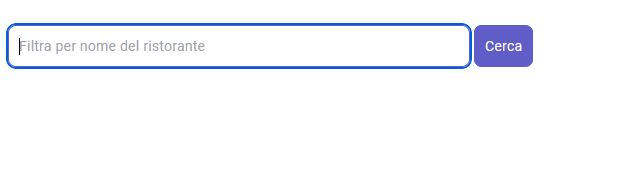
\includegraphics[width=0.5625\textwidth]{./img/Dettaglio.jpg}
            \caption{Modulo di gestione degli ingredienti}
        \end{figure}

    \subsubsection{Piatti}
    La sezione "Piatti" consente di creare e visualizzare tutti i piatti presenti nel menu del ristorante. Puoi creare un nuovo piatto utilizzando una scheda dedicata. Dopo aver cliccato sulla scheda, comparirà un modulo in cui inserire il nome del piatto, la descrizione, il prezzo e la foto del piatto.
    
        \begin{figure}[htbp]
            \centering
            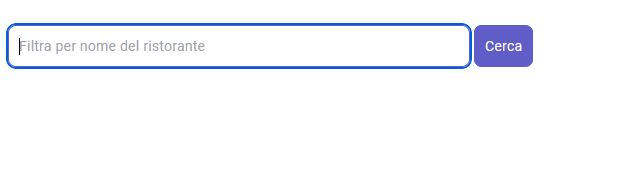
\includegraphics[width=0.5625\textwidth]{./img/Dettaglio.jpg}
            \caption{Card creazione piatto}
        \end{figure}

    \subsubsection{Aggiunta Ingredienti a un Piatto}
    Nell'elenco di tutti i piatti presenti nel menu del ristorante, è possibile visualizzare in dettaglio un piatto, semplicemente cliccando su di esso. Una volta in dettaglio, è possibile aggiungere un ingrediente per volta al piatto cliccando sul pulsante apposito in basso alla card del piatto. Si noti che per associare un ingrediente al piatto, l'ingrediente deve già esistere.
    
        \begin{figure}[htbp]
            \centering
            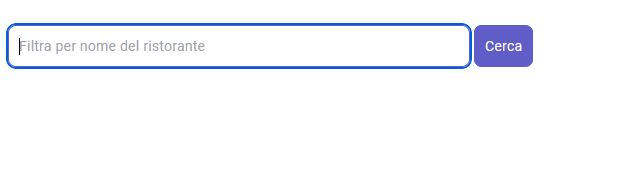
\includegraphics[width=0.5625\textwidth]{./img/Dettaglio.jpg}
            \caption{Pulsante aggiunta ingrediente ad un piatto}
        \end{figure}
        
    Inoltre, se si esegue un ulteriore click sulla card del piatto è possibile ritornare nel form, modificare i campi e salvare le modifiche, o addirittura eliminare il piatto.
    
        \begin{figure}[htbp]
            \centering
            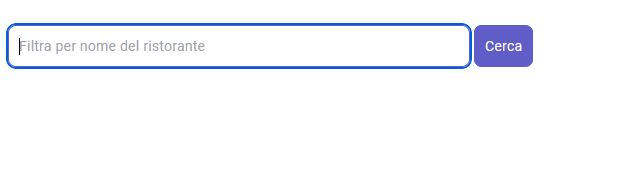
\includegraphics[width=0.5625\textwidth]{./img/Dettaglio.jpg}
            \caption{Modulo di modifica e eliminazione di un piatto}
        \end{figure}

    \subsubsection{Gestione prenotazioni}
    Tornando alla barra di navigazione, cliccando su "Prenotazioni" si accede alla pagina di gestione delle prenotazioni. Non è altro che lo stesso meccanismo che è presente nella home page del ristoratore solamente che non è presente il calendario.
